\documentclass[11pt]{article}

% Change "review" to "final" to generate the final (sometimes called camera-ready) version.
% Change to "preprint" to generate a non-anonymous version with page numbers.
\usepackage[preprint]{acl}

% Long weight-repository and blog URLs in the bibliography overrun the
% column otherwise; xurl allows a break at any character.
\usepackage{xurl}



\usepackage{xcolor}
\usepackage{pgfplots}
\pgfplotsset{compat=1.18}

% Colours for the inline figures. Names are per-figure and do not collide;
% surface/ink/muted/gridc are shared and identical everywhere.
\definecolor{fam0}{HTML}{2A78D6}
\definecolor{fam1}{HTML}{EB6834}
\definecolor{fam2}{HTML}{1BAF7A}
\definecolor{fam3}{HTML}{4A3AA7}
\definecolor{fam4}{HTML}{0B0B0B}
\definecolor{surface}{HTML}{FCFCFB}
\definecolor{ink}{HTML}{0B0B0B}
\definecolor{muted}{HTML}{52514E}
\definecolor{gridc}{HTML}{E8E7E3}
\definecolor{c0}{HTML}{1BAF7A}
\definecolor{c1}{HTML}{2A78D6}
\definecolor{c2}{HTML}{EB6834}
\definecolor{c3}{HTML}{1BAF7A}
\definecolor{c4}{HTML}{0B0B0B}
\definecolor{c5}{HTML}{EB6834}
\definecolor{s0}{HTML}{2A78D6}
\definecolor{s1}{HTML}{86B6EF}
\definecolor{s2}{HTML}{A8420C}
\definecolor{s3}{HTML}{DD6B33}
\definecolor{s4}{HTML}{EE9A6A}
\definecolor{k0}{HTML}{2A78D6}
\definecolor{k1}{HTML}{EB6834}
\definecolor{bar}{HTML}{2A78D6}
\definecolor{top}{HTML}{EB6834}
\definecolor{neg}{HTML}{E34948}
\definecolor{mid}{HTML}{F0EFEC}
\definecolor{pos}{HTML}{2A78D6}
\pgfplotsset{colormap={div}{color=(neg) color=(mid) color=(pos)}}

\newcommand{\mhcomment}[1]{\textcolor{blue}{\bf \small [ #1 --MH]}}
\newcommand{\lbcomment}[1]{\textcolor{red}{\bf \small [ #1 --LB]}}
\newcommand{\vhcomment}[1]{\textcolor{green}{\bf \small [ #1 --VH]}}

% Standard package includes
\usepackage{times}
\usepackage{latexsym}

% For proper rendering and hyphenation of words containing Latin characters (including in bib files)
\usepackage[T1]{fontenc}
% For Vietnamese characters
% \usepackage[T5]{fontenc}
% See https://www.latex-project.org/help/documentation/encguide.pdf for other character sets

% This assumes your files are encoded as UTF8
\usepackage[utf8]{inputenc}

% This is not strictly necessary, and may be commented out,
% but it will improve the layout of the manuscript,
% and will typically save some space.
\usepackage{microtype}

% This is also not strictly necessary, and may be commented out.
% However, it will improve the aesthetics of text in
% the typewriter font.
\usepackage{inconsolata}

%Including images in your LaTeX document requires adding
%additional package(s)
\usepackage{graphicx}

\usepackage{booktabs}
\usepackage{multirow}
\usepackage{xcolor}
\usepackage{array}
\usepackage{tabularx}
% If the title and author information does not fit in the area allocated, uncomment the following
%
%\setlength\titlebox{<dim>}
%
% and set <dim> to something 5cm or larger.

\title{MRL 2026 Shared Task: Latin}

% Author information can be set in various styles:
% For several authors from the same institution:
% \author{Author 1 \and ... \and Author n \\
%         Address line \ ... \ Address line}
% if the names do not fit well on one line use
%         Author 1 \ {\bf Author 2} \ ... \ {\bf Author n} \\
% For authors from different institutions:
% \author{Author 1 \ Address line \  ... \ Address line
%         \And  ... \And
%         Author n \ Address line \ ... \ Address line}
% To start a separate ``row'' of authors use \AND, as in
% \author{Author 1 \ Address line \  ... \ Address line
%         \AND
%         Author 2 \ Address line \ ... \ Address line \And
%         Author 3 \ Address line \ ... \ Address line}


% \author{Marisa Hudspeth \\
%  University of Massachusetts, Amherst \\
%  \texttt{mhudspeth@cs.umass.edu}\AND
%  Vivienne Harries-Faye \\
%  Smith College \\
%  \texttt{vharriesfaye@smith.edu} \And
%  Lee Butterman \\
%  Affiliation? no dictionaries? independent? \\
%  \texttt{leebutterman@gmail.com} }   



\author{
  \textbf{Marisa Hudspeth\textsuperscript{1}} \quad
  \textbf{Vivienne Harries-Faye\textsuperscript{2}} \quad
  \textbf{Lee Butterman\textsuperscript{3}} 
  %\\
  %\texttt{mhudspeth@cs.umass.edu} \quad \texttt{vharriesfaye@smith.edu} \quad \texttt{leebutterman@gmail.com} 
\\
 \textsuperscript{1}University of Massachusetts, Amherst \\
  \textsuperscript{2}Smith College \\
  \textsuperscript{3}NoDictionaries Labs
  \\
  \small{
    \textbf{Correspondence:} \href{mailto:mhudspeth@cs.umass.edu}{mhudspeth@cs.umass.edu}
  }
}

%\author{
%  \textbf{First Author\textsuperscript{1}},
%  \textbf{Second Author\textsuperscript{1,2}},
%  \textbf{Third T. Author\textsuperscript{1}},
%  \textbf{Fourth Author\textsuperscript{1}},
%\\
%  \textbf{Fifth Author\textsuperscript{1,2}},
%  \textbf{Sixth Author\textsuperscript{1}},
%  \textbf{Seventh Author\textsuperscript{1}},
%  \textbf{Eighth Author \textsuperscript{1,2,3,4}},
%\\
%  \textbf{Ninth Author\textsuperscript{1}},
%  \textbf{Tenth Author\textsuperscript{1}},
%  \textbf{Eleventh E. Author\textsuperscript{1,2,3,4,5}},
%  \textbf{Twelfth Author\textsuperscript{1}},
%\\
%  \textbf{Thirteenth Author\textsuperscript{3}},
%  \textbf{Fourteenth F. Author\textsuperscript{2,4}},
%  \textbf{Fifteenth Author\textsuperscript{1}},
%  \textbf{Sixteenth Author\textsuperscript{1}},
%\\
%  \textbf{Seventeenth S. Author\textsuperscript{4,5}},
%  \textbf{Eighteenth Author\textsuperscript{3,4}},
%  \textbf{Nineteenth N. Author\textsuperscript{2,5}},
%  \textbf{Twentieth Author\textsuperscript{1}}
%\\
%\\
%  \textsuperscript{1}Affiliation 1,
%  \textsuperscript{2}Affiliation 2,
%  \textsuperscript{3}Affiliation 3,
%  \textsuperscript{4}Affiliation 4,
%  \textsuperscript{5}Affiliation 5
%\\
%  \small{
%    \textbf{Correspondence:} \href{mailto:email@domain}{email@domain}
%  }
%}

\begin{document}

\maketitle
\begin{abstract}
We introduce an ECLeKTic-style QA dataset consisting of 139 questions covering cultural knowledge of Classical-era Rome. The questions are based on both primary Latin sources and secondary English sources. This dataset addresses a gap in current resources for evaluating generative models on Latin. Although Latin is well studied and has an abundance of existing NLP resources, including dictionaries, parsers, labeled data for many downstream tasks, few datasets are suited for evaluation of generative models' Latin capabilities. 
\end{abstract}

\section{Introduction}
\begin{table}[t!]
\setlength{\tabcolsep}{4pt}
\begin{tabular}{@{}p{2cm}lr@{}}
\toprule
\textbf{Macro} & \textbf{Micro Category} & \textbf{Count} \\
\midrule
\multirow{8}{*}{\parbox{2cm}{Everyday\\Life}}
  & Food, Cooking, \& Dining & 16 \\
  & Leisure & 9 \\
  & Customs & 7 \\
  & Health \& Hygiene & 7 \\
  & Clothing & 6 \\
  & Time \& Measurement & 5 \\
  & Home/Living Spaces & 1 \\
\cmidrule(l){2-3}
  & \hfill\textit{Subtotal} & \textit{51} \\
\midrule
\multirow{6}{*}{\parbox{2cm}{Power \&\\Institutions}}
  & History & 17 \\
  & Law & 11 \\
  & Money & 4 \\
  & Government & 3 \\
  & Warfare & 1 \\
\cmidrule(l){2-3}
  & \hfill\textit{Subtotal} & \textit{36} \\
\midrule
\multirow{6}{*}{\parbox{2cm}{Culture \&\\Society}}
  & Religion & 14 \\
  & Arts & 7 \\
  & Mythology & 6 \\
  & Literature & 6 \\
  & Education & 3 \\
\cmidrule(l){2-3}
  & \hfill\textit{Subtotal} & \textit{36} \\
\midrule
\multirow{4}{*}{\parbox{2cm}{Built \&\\Physical\\World}}
  & Geography & 7 \\
  & Transportation & 3 \\
  & Infra.\ \& Public Spaces & 1 \\
\cmidrule(l){2-3}
  & \hfill\textit{Subtotal} & \textit{11} \\
\midrule
\multirow{3}{*}{\parbox{2cm}{People \&\\Relationships}}
  & Love \& Courtship & 4 \\
  & Important Figures & 1 \\
\cmidrule(l){2-3}
  & \hfill\textit{Subtotal} & \textit{5} \\
\midrule
\multicolumn{2}{r}{\textbf{Total}} & \textbf{139} \\
\bottomrule
\end{tabular}
\centering
%\small
\caption{Distribution of questions by domain category.}
\label{tab:question-domains}
\end{table}

We present a Latin question-answering dataset designed to evaluate models' knowledge of Roman culture. The dataset follows the ECLeKTic framework \cite{goldman2025eclekticnovelchallengeset} and contains 139 questions covering Roman culture and history from the 6th century BCE through the 2nd century CE.\footnote{The 6th century BCE predates the period conventionally considered Classical. However, questions concerning this period cover historical knowledge that would have been relevant to and likely known by Classical-era Romans.} Questions are derived from primary sources written in Latin and secondary sources written in English.

Latin has been long-studied in academia, resulting in the creation of many linguistic resources such as dictionaries, parsers, and labeled datasets useful for morphological and syntactic analysis. These resources support the evaluation of many specific NLP tasks, but provide limited insight into how well generative models can understand and produce Latin in more open-ended settings.  

Recent work has begun to evaluate generative LLMs on specialized Latin tasks, including authorship attribution \cite{gorovaia-etal-2024-sui} and machine translation \cite{volk-etal-2024-llm}. A broader question-answering dataset has also been developed for Latin \cite{hudspeth-etal-2026-respondeoqa}. However, this dataset is bilingual Latin--English, with only a small proportion of monolingual Latin question-answer pairs. More monolingual Latin datasets are therefore needed to evaluate LLMs' Latin capabilities without relying on English as an intermediary.

Our dataset is parallel--each Latin QA pair has an equivalent English version--allowing us to to examine whether models can access the same knowledge across languages, and to disentangle language understanding from knowledge recall.


\section{Method: Dataset Creation}




\subsection{Topics}
We aimed to cover a broad range of topics related to Roman culture and history. These include everyday life, culture, society, institutions, the physical world, and people.

\subsection{Sources} \label{sec:src_description}
Because Latin is no longer a native spoken language, we cannot rely on native speakers or lived experience to identify culturally relevant knowledge. For this reason, we relied on secondary sources as well as primary sources of information.
\begin{table}[t]
\centering
\setlength{\tabcolsep}{4pt}
\begin{tabular}{@{}lr@{}}
\toprule
\textbf{Source} & \textbf{N} \\
\midrule
\textit{Primary} & \textit{70} \\
\addlinespace[3pt]
\quad Apicius, \textit{De Re Coquinaria} & 8 \\
\quad Pliny the Elder, \textit{Naturalis Historia} & 8 \\
\quad Ovid, \textit{Fasti} & 7 \\
\quad Ovid, \textit{Ars Amatoria} & 6 \\
\quad Decemviri, \textit{Lex XII Tabularum} & 5 \\
\quad Horace, \textit{Epistulae} & 4 \\
\quad Catullus, \textit{Carmina} & 4 \\
\quad Caesar, \textit{De Bello Civili} & 3 \\
\quad Caesar, \textit{De Bello Gallico} & 3 \\
\quad Cicero, \textit{Ep.\ ad Familiares} & 2 \\
\quad Martial, \textit{Apophoreta} & 2 \\
\quad Pliny the Younger, \textit{Epistulae} & 2 \\
\quad Suetonius, \textit{Divus Iulius} & 2 \\
\quad Other (14 works)\textsuperscript{\dag} & 14 \\
\midrule
\textit{Secondary} & \textit{69} \\
\addlinespace[3pt]
\quad Web & 61 \\
\quad Carcopino, \textit{Daily Life in Anc.\ Rome} & 5 \\
\quad Cowell, \textit{Everyday Life in Anc.\ Rome} & 2 \\
\quad Johnston, \textit{Priv.\ Life of the Romans} & 1 \\
\midrule
\textbf{Total} & \textbf{139} \\
\bottomrule
\end{tabular}
%\small
\caption{Distribution of questions by source.}
\label{tab:question-sources}
\vspace{2pt}
{\scriptsize \textsuperscript{\dag}One question each: Apicius, \textit{De Re Coq.}\ 3.17; Anon.\ (tit.\ par.), \textit{Inscr.\ par.\ Pomp.}; Anon.\ (tit.\ sep.), \textit{Epitaphia Romana}; Auct.\ incert., \textit{De B.\ Afr.}; Auct.\ incert., \textit{De B.\ Hisp.}; Augustine, \textit{De Civ.\ Dei}; Cicero \& Vergil, pilot; Gaius, \textit{Inst.}; Macrobius, \textit{Sat.}; Ovid, \textit{Met.}; Plautus, \textit{Amph.}; Suetonius, \textit{Div.\ Claud.}; Suetonius, \textit{Vita Hor.}; Vinidarius, \textit{Apici excerpta}.\par}
\vspace{-2mm}
\end{table}

\textbf{Primary sources:} We use ancient Latin texts as primary sources, including historical, legal, scientific, culinary, and literary works. The sources themselves date from the 5th century BCE to the early 5th century CE, although the knowledge tested by the questions concerns Roman culture and history from the 6th century BCE through the 2nd century CE. Some later sources are used as evidence for earlier Roman history and cultural practices.

\textbf{Secondary sources:} We also use modern English-language sources on Roman history, culture, and Latin, dating from 1909 to the present. These include books, scholarly resources, and web sources.


%\subsection{Regional and Time Period Variations?}
%didn't end up doing this

\subsection{Method}

We created the dataset through a combination of manual question writing and LLM-assisted question extraction. All questions were manually reviewed for relevance, factual accuracy, and quality before inclusion in the final dataset.

\paragraph{Language and Normalization}
We followed several conventions when creating and editing the dataset. We aimed to use Classical Latin throughout. Post-Classical or Neo-Latin vocabulary was replaced with Classical alternatives when possible. We removed macrons and other diacritics from all Latin text to maintain consistent orthography, and standardized numbers to be written as words rather than numerals. Answers translated into English from Latin do not preserve the Latin's case, because we prefer they sound natural in English rather than be a strict translation of the Latin. For example, the question \textit{Cuius dei imago e siligine ficta inter dona Saturnalicia editur apud Martialem?} ("The image of what god, shaped from fine wheat flour, is eaten among the Saturnalian gifts in Martial?") would naturally be answered in the genitive \textit{Priapi}, literally "of Priapus." However, in English it is more natural to simply answer in the nominative, "Priapus."

\paragraph{Sourcing Questions}
We created an initial pool of questions using two methods.

\textbf{(1) Manual question creation from secondary sources.}
We first wrote questions in English based on secondary sources. We then translated the questions into Latin using Gemini 2.5 Pro \cite{comanici2025gemini25pushingfrontier}.\footnote{We use the translation prompt from \citet{chang2026globalpiqaevaluatingcommonsense}: \texttt{``Translate the following into \{Latin\}. Do not respond to the content of the question or phrase; only translate it. Respond only with the translation, with no additional text. Text to translate: \{\}''}}
One author manually reviewed and corrected all machine translations.


We initially created 125 questions using this method. During review, we removed four questions: one duplicate and three for which the Latin translation revealed the answer and could not be easily reworded. This left 121 questions.

The machine translations generally required little correction. The average character-level Levenshtein edit distance \cite{wagner1974string} between the machine translations and their final corrected versions was 8, or 13.3\% of the machine-translated string length. Of the 121 questions, 83 required no edits.

Corrections primarily addressed vocabulary, grammar, and wording. Gemini sometimes used Post-Classical or Neo-Latin vocabulary, which we replaced with Classical alternatives (e.g., \textit{birotum} $\rightarrow$ \textit{duabus rotis instructum}). We also corrected some awkward interrogative constructions (e.g., \textit{Quis infimus honos in cursu honorum erat?} $\rightarrow$ \textit{Qui infimus honos in cursu honorum erat?}). In a small number of cases, the translation used wording that was too similar to the intended answer; where possible, we reworded the question to avoid revealing the answer (e.g. \textit{Qui parvus ruber titulus}/What small rubber tag...? $\rightarrow$ \textit{Quid parvum et rubrum}/What small, rubber thing...?  Answer: \textit{Titulus}/tag).


%We decided to normalize out macrons (\mhcomment{footnote/definition}), as Gemini inconsistently applied them when translating into Latin. 
%Some of the machine translations originally included Post-Classical or Neo-Latin vocabulary, which we swap with more Classical synonyms (e.g. \textit{birotum} $\rightarrow$ \textit{duabus rotis instructum}).
%In a few questions, the LM translation used an awkward interrogative pronoun that we changed to an interrogative adjective that agrees with the main noun (e.g. \textit{Quis infimus honos in cursu honorum erat?} $\rightarrow$ \textit{Qui infimus honos in cursu honorum erat?}).
%Some of the LM translated questions used vocabulary that was too close to the intended answer. If possible, we reworded them to not give away the answer (e.g. \textit{Qui parvus ruber titulus}/What small rubber tag...? $\rightarrow$ \textit{Quid parvum et rubrum}/What small, rubber thing...?  Answer: \textit{Titulus}/tag). 


\textbf{(2) LLM-assisted question extraction from primary sources.}
We also generated candidate question--answer pairs directly from primary Latin texts using agentic workflows with frontier models, specifically Claude Code and Opus 4.8 + Opus 5 \cite{anthropic2026opus48, anthropic2026opus5}. Primary texts were obtained from The Latin Library.\footnote{\url{https://www.thelatinlibrary.com/}}

This process produced approximately 4,000 candidate QA pairs. Because this was designed as a high-recall extraction method, many candidates did not meet the requirements of the task. In an initial manual review by one of the authors, we retained 393 questions that appeared potentially suitable. A second author then conducted a stricter review based on the task criteria, reducing this set to 112 questions. Our criteria were broadly the criteria of ECLeKTic (closed-book, entity-anchored, verifiable, decontextualizable, short-answer, translatable, non-rhetorical, culturally-salient) across a variety of hand-selected work with significant cultural value.

After the initial difficulty analysis (described later in the
\hyperref[sec:difficulty_filtering]{difficulty filtering section}), we performed an additional targeted extraction with Claude to obtain more difficult questions. This added 14 candidates, for a total of 126 questions from primary sources before final editing.

We manually reviewed these questions and corrected errors in both the Latin questions and Claude's English translations. Because the model transformed statements from the source texts into question--answer format, some outputs contained grammatical errors or depended too heavily on their original textual context. We therefore reworded questions when needed to make them self-contained, including resolving pronouns, adding relevant temporal or geographic context (e.g., ``In Ancient Rome''), and identifying the source or author when necessary (e.g., ``According to Apicius''). We also edited English translations for naturalness when they followed the Latin syntax too closely.

For the primary-source questions retained in the final dataset, the average character-level Levenshtein edit distance between Claude's Latin output and the final corrected version was 2.81 characters, or 3.5\% normalized by the original string length. For the corresponding English translations, the average edit distance was 3.47 characters, or 4.0\% normalized. These statistics are computed only over primary-source questions included in the final dataset, whereas the edit-distance statistics reported above for secondary-source questions are computed over the intermediate set of 121 questions remaining after translation review.
%Common errors: %\mhcomment{Vivienne: does this sound right? what were the typical grammar errors with the Claude translations? were they different that the Gemini translations, or about the same?}. 
%Gemini used more Neo-Latin, but this was likely due the questions being translated from English instead originally composed in Latin (as the Claude did) 

  %- trivial: grammar, esp of answers
  %- less trivial, and rare: misunderstanding the Latin
   % - question review includes does this question make sense, and the esoterica are less interesting to include, and we as experts in the field know what's up
%- rewording of source text to transform into a QA pair: What has to be changed? grammatical constructions, case of the answer, decontextualizing/making standalone (pronoun resolution; for questions about literature, adding info about the source text/author)
%  - [to marisa and vivienne: do we want to standardize into full prep phrases/sentences/etc for answers?]


\paragraph{Exclusion Criteria}

We excluded questions that did not fit the scope or goals of the shared task. In particular, we removed questions that:

\begin{itemize}
\vspace{-2mm}
\item were too obscure or unlikely to represent broadly shared cultural knowledge;
\vspace{-3mm}
\item depended too heavily on a specific non-landmark source, such as questions about plot details, individual passages, or an author's personal opinions;
\vspace{-3mm}
\item required answers longer than a few words;
\vspace{-3mm}
\item had multiple equally valid answers;
\vspace{-3mm}
\item fell too far outside our approximate time range of the 6th century BCE through the 2nd century CE;
\vspace{-3mm}
\item concerned cultural practices or facts that were not distinctive to Roman culture, even if they appeared in Roman sources;
\vspace{-3mm}
\item focused primarily on non-Roman peoples, cultures, or historical events;
\vspace{-3mm}
\item were duplicative, either directly or by testing nearly the same knowledge as another question;
\vspace{-3mm}
\item were too easy based on human difficulty annotations and model performance; or
\vspace{-3mm}
\item did not contribute to the desired balance of topics and difficulty levels in the final dataset.
\end{itemize}

\begin{table}[t]
\centering
\setlength{\tabcolsep}{5pt}
\begin{tabularx}{\linewidth}{@{}X X@{}}
\toprule
\textbf{Excluded question} & \textbf{Reason} \\
\midrule
%What oil does the \textit{pullus leucozomus} (`white-broth chicken') receive in abundance in Apicius? & Too specific to an individual recipe rather than a broader Roman culinary practice. \\
%\addlinespace
What does Catullus feel himself doing at once, not knowing why, in his most famous couplet? & Depends on recall of a specific literary passage rather than broader cultural knowledge. \\ \hline
\addlinespace
What kind of vehicle is the summoner not obliged to furnish for a sick man he has summoned, under the Law of the Twelve Tables? & Too specific and unlikely to represent broadly shared cultural knowledge. \\\hline
\addlinespace
What animal nursed the exposed twins Romulus and Remus? & Too easy; the answer (\textit{she-wolf}) is widely known. \\\hline
\addlinespace
On every which day does Tacitus report that the Jews keep rest? & Tests a cultural practice that is not distinctive to Roman culture and remains widely known today. \\\hline
\addlinespace
What does a patron become under the Law of the Twelve Tables if he has wronged his client? & Allows multiple valid answers or descriptions (e.g., \textit{sacer}, ``accursed,'' ``forfeited to the gods,'' or ``outlawed''). \\\hline
\addlinespace
What title did the plebs, the senate, and the knights confer on Augustus on the Nones of February, as Ovid sings in the \textit{Fasti}? & Duplicative of another question testing the title \textit{pater patriae}. \\
\bottomrule
\end{tabularx}
\caption{Examples of questions excluded during dataset filtering.}
\label{tab:exclusion-examples}
\end{table}
Table~\ref{tab:exclusion-examples} gives examples of questions removed during filtering.

%For example, we exclude:
%“What oil does the pullus leucozomus ('white-broth chicken') receive in abundance in Apicius?” This asks about a specific personal recipe rather than a general cooking convention. 
%“What does Catullus feel himself doing at once, not knowing why, in his most famous couplet?” - This is reliant on one specific source and does not include enough valuable cultural information. This tests recall of a specific sentence or line in a piece of literature.
%“What kind of vehicle is the summoner not obliged to furnish for a sick man he has summoned, under the Law of the Twelve Tables?’ This is too specific and falls outside the scope of what an Ancient Roman citizen could reasonably be expected to know. 

\paragraph{Difficulty Calibration and Filtering} \label{sec:difficulty_filtering}

\mhcomment{question instructions in Latin on how to respond (short)}
\mhcomment{llm as judge is few shot}

When creating the dataset, we found it difficult to balance culturally salient questions with appropriate difficulty. Questions about common aspects of Roman culture were often too easy for current language models, while more difficult questions were sometimes highly specific and did not fit the shared-task criterion that the knowledge should plausibly be familiar to members of the relevant cultural or linguistic community.

We therefore assessed question difficulty in two ways. First, we manually assigned each question to one of four difficulty levels:

\begin{itemize}
    \vspace{-2mm}
    \item \textcolor{red!85!black}{\textbf{Red}}: a Classicist may not know the answer off the top of their head.
    \vspace{-3mm}
    \item \textcolor{orange!90!black}{\textbf{Orange}}: an upper-level Classics student or scholar would probably know the answer.
    \vspace{-3mm}
    \item \textcolor{blue!80!black}{\textbf{Blue}}: a beginner Latin student would probably know the answer.
    \vspace{-3mm}
    \item \textcolor{green!60!black}{\textbf{Green}}: a middle-school world history student would probably know the answer.
\end{itemize}

\begin{table}[t]
\centering
\small
\setlength{\tabcolsep}{3pt}
\begin{tabular}{@{}lrrrr@{}}
\toprule
\textbf{Model} &
\textcolor{green!60!black}{\textbf{Green}} &
\textcolor{blue!80!black}{\textbf{Blue}} &
\textcolor{orange!90!black}{\textbf{Orange}} &
\textcolor{red!85!black}{\textbf{Red}} \\
\midrule
Gemma 4 E2B           & 52.0  & 44.3 & 17.9 & 11.6 \\
Gemma 4 31B           & 100.0 & 97.1 & 80.0 & 60.5 \\
GPT-OSS 120B          & 100.0 & 90.0 & 74.7 & 51.2 \\
Nemotron 3 Super 120B & 100.0 & 95.7 & 86.3 & 81.4 \\
\midrule
\textbf{N questions}            & 25    & 70   & 95   & 43   \\
\bottomrule
\end{tabular}
\caption{Pass@any accuracy (\%) by manually annotated difficulty level for the 233 questions evaluated at this stage. Each model was sampled three times per question; a question is counted as correct if at least one of the three responses was judged correct by GPT-OSS 120B. }
\label{tab:difficulty-models}
\vspace{-5mm}
\end{table}

Second, we evaluated the 233 questions remaining (121 secondary, 112 primary) after the initial sourcing and manual filtering stages using several open-source language models ranging from approximately 2B to 120B parameters \cite{gemmateam2026gemma4technicalreport, openai2025gptoss, chandiramani2026nemotron}. Each model was sampled three times per question. We report \texttt{pass@any}, which counts a question as correct if at least one of the three responses was judged correct by GPT-OSS 120B \cite{openai2025gptoss}.

The manually assigned difficulty levels aligned closely with model performance
(Table~\ref{tab:difficulty-models}). For every model, \texttt{pass@any} accuracy decreased monotonically from green to blue to orange to red questions. Treating the four human annotations as an ordinal measure of question ease, their Pearson correlation with aggregate \texttt{pass@any} accuracy ranged from $r=0.96$ to $r=0.99$ across models.\footnote{Ease was coded from 4 (green, easiest) to 1 (red, most difficult);
correlations are computed over the four aggregate difficulty levels.}

%3) We score each question for difficulty, manually, based on expert opinion.

%4) We make a straightforward question answering harness with DSPy and various open source models from 0.5B to 31B parameters, and we answer for each question with 3 rollouts. \mhcomment{need to cite exact models; is there a system prompt or anything other than just asking the question? hyperparameters--I assume whatever the defaults are}

%5) We find that our handmade analysis for difficulty correlates (corr coeff 0.FIXMETODO) with how much easier a question is for a smaller LLM (under 4B parameters) vs a larger LLM (over 10B parameters), and we find that this generalizes across a variety of models, with thinking on and off.

%6) We co-designed our dataset with LLMs: we first compiled many questions that were culturally salient, and then found that LLMs for edge AI (gemma 4, qwen3:4b) answer these questions correctly, and we pruned our questions for difficulty.
\begin{table*}[t!]
\centering
%\small
\setlength{\tabcolsep}{3pt}
\begin{tabular}{@{}>{\raggedright\arraybackslash}p{2cm}p{3cm}p{9.5cm}@{}}
\toprule
\textbf{Category} & \textbf{Source} & \textbf{Question \& Answer} \\
\midrule
Everyday Life \newline {\small(Food, Cooking, \& Dining)}
& Apicius, \textit{De Re Coq.}\ 6.8.11
& \textbf{Q:} Quo nomine ius pulli Vardani, lacte et albamentis ovorum confectum, apud Apicium appellatur? \textit{[By what name is the sauce of the pullus Vardanus, made with milk and egg whites, called in Apicius?]} \newline
\textbf{A:} Ius candidum \textit{[White sauce]} \\
\midrule
Everyday Life \newline {\small(Leisure)}
& penelope .uchicago.edu
& \textbf{Q:} Quid est nomen vict\=us Gladiatorum Romanorum? \textit{[What is the name for the diet of Roman gladiators?]} \newline
\textbf{A:} Sagina Gladitoria \textit{[Sagina Gladitoria]} \\
\midrule
Power \& Institutions\ \newline {\small(History)}
& Suetonius, \textit{Div.\ Iul.}\ 56
& \textbf{Q:} Quam litteram Caesar in notis suis pro A scribebat? \textit{[Which letter did Caesar write in place of A in his cipher?]} \newline
\textbf{A:} D \textit{[D]} \\
\midrule
Power \& Institutions\ \newline {\small(Government)}
& en.wikipedia.org
& \textbf{Q:} In qua sella solis magistratibus cum imperio sedere licet? \textit{[What chair are only magistrates holding Imperium allowed to sit on?]} \newline
\textbf{A:} Sella curulis \textit{[Curule seat]} \\
\midrule
Culture \& Society\ \newline {\small(Religion)}
& Ovid, \textit{Fasti} 3.141--144
& \textbf{Q:} Quo die ignis novus in arcana Vestae aede fieri dicitur? \textit{[On what day is the new fire said to be kindled in the inner shrine of Vesta?]} \newline
\textbf{A:} Kalendis Martiis \textit{[Kalends of March]} \\
\midrule
Culture \& Society\ \newline {\small(Education)}
& en.wiktionary.org
& \textbf{Q:} Quod est nomen magistri ludi qui pueros Romanos parvos prima elementa legendi, scribendi, ratiocinandique docebat? \textit{[What is the name of the school teacher who taught young Roman children basic reading, writing, and arithmetic?]} \newline
\textbf{A:} Litterator \textit{[Litterator]} \\
\midrule
Built \& Phys.\ World \newline {\small(Geography)}
& Caesar, \textit{De B.\ Gall.}\ 5.11
& \textbf{Q:} Quod flumen, ut Caesar scribit, fines Cassivellauni a maritimis civitatibus dividit? \textit{[Which river, as Caesar writes, divides the territory of Cassivellaunus from the maritime states?]} \newline
\textbf{A:} Tamesis \textit{[Thames]} \\
\midrule
Built \& Phys.\ World \newline {\small(Geography)}
& en.wikipedia.org
& \textbf{Q:} Quod fretum provinciam Hispaniam ab ora Mauretaniae dividit? \textit{[What body of water separates the province of Hispania from the coast of Mauretania?]} \newline
\textbf{A:} Fretum Gaditanum \textit{[Strait of Gibraltar]} \\
\midrule
People \& Rel.\ \newline {\small(Love \& Courtship)}
& europe \newline .factsanddetails .com
& \textbf{Q:} Quis puer patrimus et matrimus cumerum in pompa nuptiali fert? \textit{[What boy, required to have both parents living, carries the offering basket in a Roman wedding procession?]} \newline
\textbf{A:} Camillus \textit{[Camillus]} \\
\bottomrule
\end{tabular}
\caption{Example questions from the dataset, including both primary and secondary sources. Under category, the macro category is listed first with the micro category in parentheses. English versions of questions and answers are [\textit{bracketed and italicized}]}.
\label{tab:example-questions}
\end{table*}
Based on these results, we dropped all green and most blue questions from the final dataset. We then identified questions at the extremes of the difficulty distribution for further review.


From a set of the 32 most difficult questions--those that a medium-sized open source model (Qwen 3.6 27B \cite{qwen3.6-27b}) missed on 3/3 attempts--we kept two blue questions and no green. Some orange and red questions in this set were dropped or reworded, as we found that models answered incorrectly due to question ambiguity rather than genuine difficulty.



From a set of the 38 easiest questions--those that a small open source model (Gemma 4 E2B) answered correctly on 3/3 attempts--we filtered out eight orange and red questions. Two orange questions were kept after rewording them to increase the difficulty.

The final dataset consists of 89 questions manually classified as orange-level difficulty, 48 red, and 2 blue.




\section{Dataset Description}
%Number of questions
%Distribution of topics
%Distribution of sources (originally in Latin text, or in English text about Latin/Rome? date of publication of sources?)
%Percent manually created, versus percent scraped with Claude
%Distribution of time period/region-specific questions?
%\begin{table}[t]
\centering
\setlength{\tabcolsep}{4pt}
\begin{tabular}{@{}lr@{}}
\toprule
\textbf{Source} & \textbf{N} \\
\midrule
\textit{Primary} & \textit{70} \\
\addlinespace[3pt]
\quad Apicius, \textit{De Re Coquinaria} & 8 \\
\quad Pliny the Elder, \textit{Naturalis Historia} & 8 \\
\quad Ovid, \textit{Fasti} & 7 \\
\quad Ovid, \textit{Ars Amatoria} & 6 \\
\quad Decemviri, \textit{Lex XII Tabularum} & 5 \\
\quad Horace, \textit{Epistulae} & 4 \\
\quad Catullus, \textit{Carmina} & 4 \\
\quad Caesar, \textit{De Bello Civili} & 3 \\
\quad Caesar, \textit{De Bello Gallico} & 3 \\
\quad Cicero, \textit{Ep.\ ad Familiares} & 2 \\
\quad Martial, \textit{Apophoreta} & 2 \\
\quad Pliny the Younger, \textit{Epistulae} & 2 \\
\quad Suetonius, \textit{Divus Iulius} & 2 \\
\quad Other (14 works)\textsuperscript{\dag} & 14 \\
\midrule
\textit{Secondary} & \textit{69} \\
\addlinespace[3pt]
\quad Web & 61 \\
\quad Carcopino, \textit{Daily Life in Anc.\ Rome} & 5 \\
\quad Cowell, \textit{Everyday Life in Anc.\ Rome} & 2 \\
\quad Johnston, \textit{Priv.\ Life of the Romans} & 1 \\
\midrule
\textbf{Total} & \textbf{139} \\
\bottomrule
\end{tabular}
%\small
\caption{Distribution of questions by source.}
\label{tab:question-sources}
\vspace{2pt}
{\scriptsize \textsuperscript{\dag}One question each: Apicius, \textit{De Re Coq.}\ 3.17; Anon.\ (tit.\ par.), \textit{Inscr.\ par.\ Pomp.}; Anon.\ (tit.\ sep.), \textit{Epitaphia Romana}; Auct.\ incert., \textit{De B.\ Afr.}; Auct.\ incert., \textit{De B.\ Hisp.}; Augustine, \textit{De Civ.\ Dei}; Cicero \& Vergil, pilot; Gaius, \textit{Inst.}; Macrobius, \textit{Sat.}; Ovid, \textit{Met.}; Plautus, \textit{Amph.}; Suetonius, \textit{Div.\ Claud.}; Suetonius, \textit{Vita Hor.}; Vinidarius, \textit{Apici excerpta}.\par}
\vspace{-2mm}
\end{table}
%\begin{table}[t!]
\setlength{\tabcolsep}{4pt}
\begin{tabular}{@{}p{2cm}lr@{}}
\toprule
\textbf{Macro} & \textbf{Micro Category} & \textbf{Count} \\
\midrule
\multirow{8}{*}{\parbox{2cm}{Everyday\\Life}}
  & Food, Cooking, \& Dining & 16 \\
  & Leisure & 9 \\
  & Customs & 7 \\
  & Health \& Hygiene & 7 \\
  & Clothing & 6 \\
  & Time \& Measurement & 5 \\
  & Home/Living Spaces & 1 \\
\cmidrule(l){2-3}
  & \hfill\textit{Subtotal} & \textit{51} \\
\midrule
\multirow{6}{*}{\parbox{2cm}{Power \&\\Institutions}}
  & History & 17 \\
  & Law & 11 \\
  & Money & 4 \\
  & Government & 3 \\
  & Warfare & 1 \\
\cmidrule(l){2-3}
  & \hfill\textit{Subtotal} & \textit{36} \\
\midrule
\multirow{6}{*}{\parbox{2cm}{Culture \&\\Society}}
  & Religion & 14 \\
  & Arts & 7 \\
  & Mythology & 6 \\
  & Literature & 6 \\
  & Education & 3 \\
\cmidrule(l){2-3}
  & \hfill\textit{Subtotal} & \textit{36} \\
\midrule
\multirow{4}{*}{\parbox{2cm}{Built \&\\Physical\\World}}
  & Geography & 7 \\
  & Transportation & 3 \\
  & Infra.\ \& Public Spaces & 1 \\
\cmidrule(l){2-3}
  & \hfill\textit{Subtotal} & \textit{11} \\
\midrule
\multirow{3}{*}{\parbox{2cm}{People \&\\Relationships}}
  & Love \& Courtship & 4 \\
  & Important Figures & 1 \\
\cmidrule(l){2-3}
  & \hfill\textit{Subtotal} & \textit{5} \\
\midrule
\multicolumn{2}{r}{\textbf{Total}} & \textbf{139} \\
\bottomrule
\end{tabular}
\centering
%\small
\caption{Distribution of questions by domain category.}
\label{tab:question-domains}
\end{table}
%\begin{table*}[t!]
\centering
%\small
\setlength{\tabcolsep}{3pt}
\begin{tabular}{@{}>{\raggedright\arraybackslash}p{2cm}p{3cm}p{9.5cm}@{}}
\toprule
\textbf{Category} & \textbf{Source} & \textbf{Question \& Answer} \\
\midrule
Everyday Life \newline {\small(Food, Cooking, \& Dining)}
& Apicius, \textit{De Re Coq.}\ 6.8.11
& \textbf{Q:} Quo nomine ius pulli Vardani, lacte et albamentis ovorum confectum, apud Apicium appellatur? \textit{[By what name is the sauce of the pullus Vardanus, made with milk and egg whites, called in Apicius?]} \newline
\textbf{A:} Ius candidum \textit{[White sauce]} \\
\midrule
Everyday Life \newline {\small(Leisure)}
& penelope .uchicago.edu
& \textbf{Q:} Quid est nomen vict\=us Gladiatorum Romanorum? \textit{[What is the name for the diet of Roman gladiators?]} \newline
\textbf{A:} Sagina Gladitoria \textit{[Sagina Gladitoria]} \\
\midrule
Power \& Institutions\ \newline {\small(History)}
& Suetonius, \textit{Div.\ Iul.}\ 56
& \textbf{Q:} Quam litteram Caesar in notis suis pro A scribebat? \textit{[Which letter did Caesar write in place of A in his cipher?]} \newline
\textbf{A:} D \textit{[D]} \\
\midrule
Power \& Institutions\ \newline {\small(Government)}
& en.wikipedia.org
& \textbf{Q:} In qua sella solis magistratibus cum imperio sedere licet? \textit{[What chair are only magistrates holding Imperium allowed to sit on?]} \newline
\textbf{A:} Sella curulis \textit{[Curule seat]} \\
\midrule
Culture \& Society\ \newline {\small(Religion)}
& Ovid, \textit{Fasti} 3.141--144
& \textbf{Q:} Quo die ignis novus in arcana Vestae aede fieri dicitur? \textit{[On what day is the new fire said to be kindled in the inner shrine of Vesta?]} \newline
\textbf{A:} Kalendis Martiis \textit{[Kalends of March]} \\
\midrule
Culture \& Society\ \newline {\small(Education)}
& en.wiktionary.org
& \textbf{Q:} Quod est nomen magistri ludi qui pueros Romanos parvos prima elementa legendi, scribendi, ratiocinandique docebat? \textit{[What is the name of the school teacher who taught young Roman children basic reading, writing, and arithmetic?]} \newline
\textbf{A:} Litterator \textit{[Litterator]} \\
\midrule
Built \& Phys.\ World \newline {\small(Geography)}
& Caesar, \textit{De B.\ Gall.}\ 5.11
& \textbf{Q:} Quod flumen, ut Caesar scribit, fines Cassivellauni a maritimis civitatibus dividit? \textit{[Which river, as Caesar writes, divides the territory of Cassivellaunus from the maritime states?]} \newline
\textbf{A:} Tamesis \textit{[Thames]} \\
\midrule
Built \& Phys.\ World \newline {\small(Geography)}
& en.wikipedia.org
& \textbf{Q:} Quod fretum provinciam Hispaniam ab ora Mauretaniae dividit? \textit{[What body of water separates the province of Hispania from the coast of Mauretania?]} \newline
\textbf{A:} Fretum Gaditanum \textit{[Strait of Gibraltar]} \\
\midrule
People \& Rel.\ \newline {\small(Love \& Courtship)}
& europe \newline .factsanddetails .com
& \textbf{Q:} Quis puer patrimus et matrimus cumerum in pompa nuptiali fert? \textit{[What boy, required to have both parents living, carries the offering basket in a Roman wedding procession?]} \newline
\textbf{A:} Camillus \textit{[Camillus]} \\
\bottomrule
\end{tabular}
\caption{Example questions from the dataset, including both primary and secondary sources. Under category, the macro category is listed first with the micro category in parentheses. English versions of questions and answers are [\textit{bracketed and italicized}]}.
\label{tab:example-questions}
\end{table*}

The final dataset contains 139 questions, split almost evenly between primary and secondary sources (Table \ref{tab:question-sources}).

Most questions fall under Everyday Life (51), Power and Institutions (36), and Culture and Society (36) (see Table \ref{tab:question-domains}). The largest sub-categories are History (17); Food, Cooking, and Dining (16); Religion (14); and Law (11).

Table ~\ref{tab:example-questions} shows a sample of questions from the dataset across every macro-category and source type.


\section{Results}

We ran our final dataset of questions through over a dozen open-source models, spanning parameter counts from 0.5B to 31B, thinking and non thinking, across multiple families: Gemma4, E2B/12B/31B \cite{gemmateam2026gemma4technicalreport,gemma4-e2b-weights,gemma4-12b-weights,gemma4-31b-weights}; LiquidAI's LFM2.5, 230M/2.6B \cite{lfm25-announcement,liquidai2025lfm2,lfm25-230m-gguf,lfm25-26b-gguf}; Qwen2.5, 0.5B/1.5B/3B/7B/32B \cite{qwen25-report,qwen25-collection}; Qwen3, 4B/30B-A3B, Instruct/Thinking, 2507 edition \cite{qwen3-techreport,qwen3-4b-instruct-2507-weights,qwen3-4b-thinking-2507-weights,qwen3-30b-a3b-instruct-2507-weights,qwen3-30b-a3b-thinking-2507-weights}; and Qwen3.6 27B \cite{qwen3.6-27b,qwen36-27b-weights}. We use 4-bit precision for inference on the larger models; the largest, Gemma4 31B, is 20GB. Modern phones can run Qwen3 4B and Gemma4 E2B. Our harness is open-source ( https://github.com/lsb/latin-q-and-a ) and uses DSPy for 4-shot question answering. The harness asks questions in Latin and uses an LLM as judge (string matching fails to account for correct answers in an incorrect case).

Latin is well understood by small models. Thirty-billion parameter models from 2026 have a pass@3 rate of over 75\% on this cultural question dataset. Even models designed for edge-AI tool routing have enough world knowledge to correctly answer many cultural questions. Many models differ in consistency between runs (Figure~\ref{fig:consistency}), and similar pass@3 performance can represent a wide spread of similarly-wrong versus differently-wrong answers for the questions answered incorrectly.

LLMs are often trained on an abundance of training data from the internet. Many LLMs are trained on originals and translations of Latin texts, as well as many of the sources of our manually-compiled questions. Excluding the models under 4B parameters, which do not get 10\% of the questions correct, questions extracted from texts have a significantly lower percentage correct, across all sizes of model and all model families, up to 24 percentage points in the middle of the range. (Figure~\ref{fig:provenance-split}).

Accuracy also varies by subject (Figure~\ref{fig:category-knowledge}), from 46\% on Geography to 16\% on Customs.

The larger Qwen and Gemma models largely miss the same questions as each other (Figure~\ref{fig:co-failure}), which suggests one dominant axis of difficulty across multiple training regimens and multiple sources of training data.

Future directions include tool use for Wikipedia and corpus browsing, to test if smaller models are able to improve their scores not only by thinking tokens but also by explicit corpora.

\begin{figure}[t]
  \centering
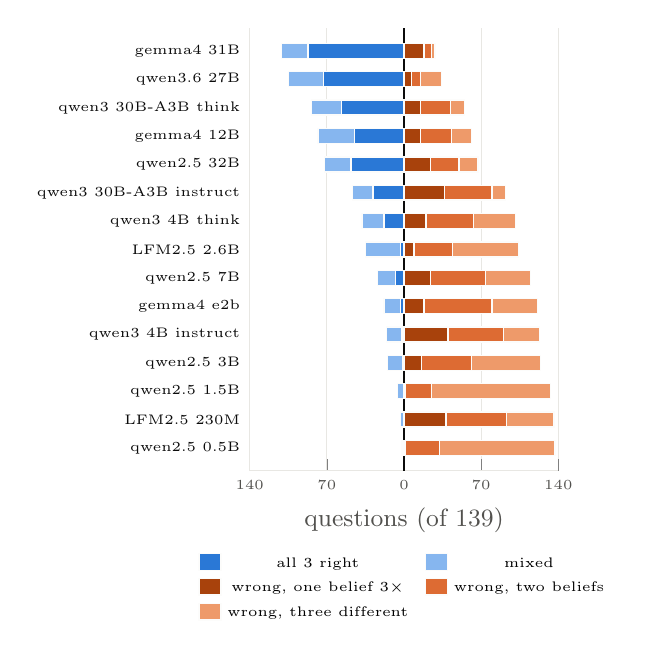
\begin{tikzpicture}
\begin{axis}[
  width=5.5cm, height=7.2cm,
  xbar stacked, bar width=5.4pt,
  xmin=-140, xmax=140, ymin=-0.8, ymax=14.8,
  xlabel={questions (of 139)},
  xlabel style={font=\small, color=muted},
  tick label style={font=\tiny, color=muted},
  ytick={0,1,2,3,4,5,6,7,8,9,10,11,12,13,14},
  yticklabels={gemma4 31B,qwen3.6 27B,qwen3 30B-A3B think,gemma4 12B,qwen2.5 32B,qwen3 30B-A3B instruct,qwen3 4B think,LFM2.5 2.6B,qwen2.5 7B,gemma4 e2b,qwen3 4B instruct,qwen2.5 3B,qwen2.5 1.5B,LFM2.5 230M,qwen2.5 0.5B},
  y dir=reverse, ytick style={draw=none},
  yticklabel style={font=\tiny, color=ink},
  xmajorgrids, grid style={gridc, line width=0.3pt},
  axis line style={gridc}, axis x line*=bottom, axis y line*=left,
  legend style={draw=none, font=\tiny, at={(0.5,-0.17)}, anchor=north, legend columns=2, /tikz/every even column/.append style={column sep=4pt}},
  xtick={-140,-70,0,70,140},
  xticklabels={140,70,0,70,140},
]
\addplot[fill=s0, draw=surface, line width=0.5pt] coordinates {(-87,0) (-73,1) (-57,2) (-45,3) (-48,4) (-28,5) (-18,6) (-3,7) (-8,8) (-3,9) (-2,10) (-1,11) (0,12) (0,13) (0,14)};
\addlegendentry{all 3 right}
\addplot[fill=s1, draw=surface, line width=0.5pt] coordinates {(-24,0) (-32,1) (-27,2) (-33,3) (-24,4) (-19,5) (-20,6) (-32,7) (-16,8) (-15,9) (-14,10) (-14,11) (-6,12) (-3,13) (-2,14)};
\addlegendentry{mixed}
\addplot[fill=s2, draw=surface, line width=0.5pt] coordinates {(18,0) (7,1) (15,2) (15,3) (24,4) (37,5) (20,6) (9,7) (24,8) (18,9) (40,10) (16,11) (1,12) (38,13) (1,14)};
\addlegendentry{wrong, one belief 3$\times$}
\addplot[fill=s3, draw=surface, line width=0.5pt] coordinates {(7,0) (8,1) (27,2) (28,3) (26,4) (43,5) (43,6) (35,7) (50,8) (62,9) (50,10) (45,11) (24,12) (55,13) (31,14)};
\addlegendentry{wrong, two beliefs}
\addplot[fill=s4, draw=surface, line width=0.5pt] coordinates {(3,0) (19,1) (13,2) (18,3) (17,4) (12,5) (38,6) (60,7) (41,8) (41,9) (33,10) (63,11) (108,12) (43,13) (105,14)};
\addlegendentry{wrong, three different}
\draw[ink, line width=1pt] (axis cs:0,-0.8) -- (axis cs:0,14.8);
\end{axis}
\end{tikzpicture}
  \caption{Agreement across the three samples of each question. Left of the center line, the model answered correctly at least once, and dark blue is unanimity. Right of the center line, the model answered incorrectly, and the darker the shading the more consistent the wrong answer was. Using LLM as a judge.}
  \label{fig:consistency}
\end{figure}


\begin{figure}[t]
  \centering
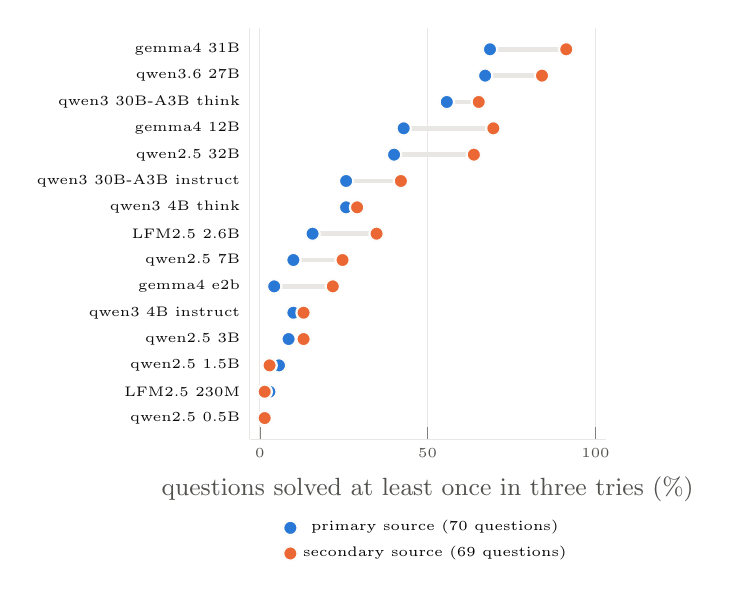
\begin{tikzpicture}
\begin{axis}[
  width=6.1cm, height=6.8cm,
  xlabel={questions solved at least once in three tries (\%)},
  xlabel style={font=\small, color=muted},
  tick label style={font=\tiny, color=muted},
  xmin=-3, xmax=103, ymin=-0.8, ymax=14.8,
  ytick={0,1,2,3,4,5,6,7,8,9,10,11,12,13,14},
  yticklabels={gemma4 31B,qwen3.6 27B,qwen3 30B-A3B think,gemma4 12B,qwen2.5 32B,qwen3 30B-A3B instruct,qwen3 4B think,LFM2.5 2.6B,qwen2.5 7B,gemma4 e2b,qwen3 4B instruct,qwen2.5 3B,qwen2.5 1.5B,LFM2.5 230M,qwen2.5 0.5B},
  y dir=reverse, ytick style={draw=none},
  yticklabel style={font=\tiny, color=ink},
  xmajorgrids, grid style={gridc, line width=0.3pt},
  axis line style={gridc}, axis x line*=bottom, axis y line*=left,
  legend style={draw=none, font=\tiny, at={(0.5,-0.17)}, anchor=north, legend columns=1},
]
\addplot[gridc, line width=1.6pt, forget plot] coordinates {(68.57,0) (91.30,0)};
\addplot[gridc, line width=1.6pt, forget plot] coordinates {(67.14,1) (84.06,1)};
\addplot[gridc, line width=1.6pt, forget plot] coordinates {(55.71,2) (65.22,2)};
\addplot[gridc, line width=1.6pt, forget plot] coordinates {(42.86,3) (69.57,3)};
\addplot[gridc, line width=1.6pt, forget plot] coordinates {(40.00,4) (63.77,4)};
\addplot[gridc, line width=1.6pt, forget plot] coordinates {(25.71,5) (42.03,5)};
\addplot[gridc, line width=1.6pt, forget plot] coordinates {(25.71,6) (28.99,6)};
\addplot[gridc, line width=1.6pt, forget plot] coordinates {(15.71,7) (34.78,7)};
\addplot[gridc, line width=1.6pt, forget plot] coordinates {(10.00,8) (24.64,8)};
\addplot[gridc, line width=1.6pt, forget plot] coordinates {(4.29,9) (21.74,9)};
\addplot[gridc, line width=1.6pt, forget plot] coordinates {(10.00,10) (13.04,10)};
\addplot[gridc, line width=1.6pt, forget plot] coordinates {(8.57,11) (13.04,11)};
\addplot[gridc, line width=1.6pt, forget plot] coordinates {(5.71,12) (2.90,12)};
\addplot[gridc, line width=1.6pt, forget plot] coordinates {(2.86,13) (1.45,13)};
\addplot[gridc, line width=1.6pt, forget plot] coordinates {(1.43,14) (1.45,14)};
\addplot[only marks, mark=*, mark size=2.6pt, mark options={fill=k0, draw=surface, line width=0.8pt}] coordinates {(68.57,0) (67.14,1) (55.71,2) (42.86,3) (40.00,4) (25.71,5) (25.71,6) (15.71,7) (10.00,8) (4.29,9) (10.00,10) (8.57,11) (5.71,12) (2.86,13) (1.43,14)};
\addlegendentry{primary source (70 questions)}
\addplot[only marks, mark=*, mark size=2.6pt, mark options={fill=k1, draw=surface, line width=0.8pt}] coordinates {(91.30,0) (84.06,1) (65.22,2) (69.57,3) (63.77,4) (42.03,5) (28.99,6) (34.78,7) (24.64,8) (21.74,9) (13.04,10) (13.04,11) (2.90,12) (1.45,13) (1.45,14)};
\addlegendentry{secondary source (69 questions)}
\end{axis}
\end{tikzpicture}
  \caption{Accuracy on primary-source questions (extracted from a Latin text) against secondary-source questions (written from an English citation), for each model. The figure beside each pair is the difference in points. The gap is near zero for the weakest models and reaches 24 points in the middle of the range.}
  \label{fig:provenance-split}
\end{figure}

\begin{figure}[t]
  \centering
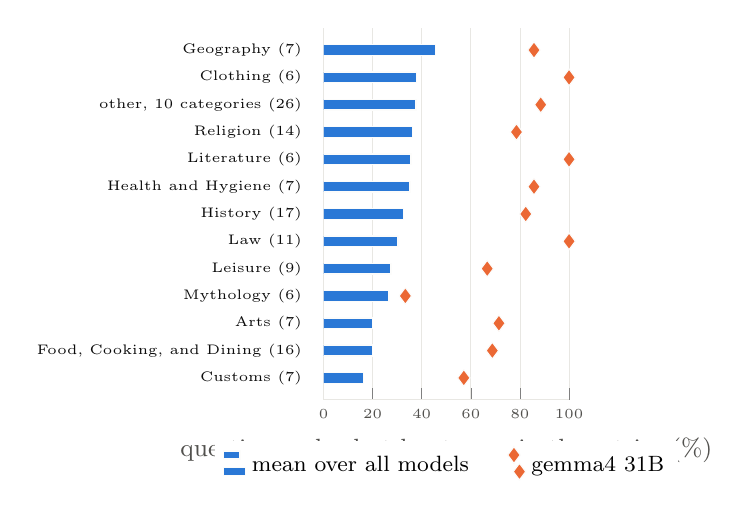
\begin{tikzpicture}
\begin{axis}[
  width=4.7cm, height=6.3cm, xbar, bar width=3.9pt,
  xlabel={questions solved at least once in three tries (\%)},
  xlabel style={font=\small, color=muted},
  tick label style={font=\tiny, color=muted},
  xmin=0, xmax=100, ymin=-0.8, ymax=12.8,
  ytick={0,1,2,3,4,5,6,7,8,9,10,11,12},
  yticklabels={{Customs  (7)},{Food, Cooking, and Dining  (16)},{Arts  (7)},{Mythology  (6)},{Leisure  (9)},{Law  (11)},{History  (17)},{Health and Hygiene  (7)},{Literature  (6)},{Religion  (14)},{other, 10 categories  (26)},{Clothing  (6)},{Geography  (7)}},
  ytick style={draw=none},
  yticklabel style={font=\tiny, color=ink},
  xmajorgrids, grid style={gridc, line width=0.3pt},
  axis line style={gridc}, axis x line*=bottom, axis y line*=left,
  legend style={draw=none, font=\footnotesize, at={(0.5,-0.11)}, anchor=north, legend columns=2, /tikz/every even column/.append style={column sep=12pt}},
]
\addplot[fill=bar, draw=surface, line width=0.5pt] coordinates {(16.19,0) (20.00,1) (20.00,2) (26.67,3) (27.41,4) (30.30,5) (32.55,6) (35.24,7) (35.56,8) (36.19,9) (37.69,10) (37.78,11) (45.71,12)};
\addlegendentry{mean over all models}
\addplot[only marks, mark=diamond*, mark size=3pt, mark options={fill=top, draw=surface}] coordinates {(57.14,0) (68.75,1) (71.43,2) (33.33,3) (66.67,4) (100.00,5) (82.35,6) (85.71,7) (100.00,8) (78.57,9) (88.46,10) (100.00,11) (85.71,12)};
\addlegendentry{gemma4 31B}
\end{axis}
\end{tikzpicture}
  \caption{Accuracy by subject category. Bars are the mean over all models and the diamond is Gemma4 31B. The figure after each subject is how many questions it rests on; categories with fewer than six questions are pooled into one row.}
  \label{fig:category-knowledge}
\end{figure}

\begin{figure}[t]
  \centering
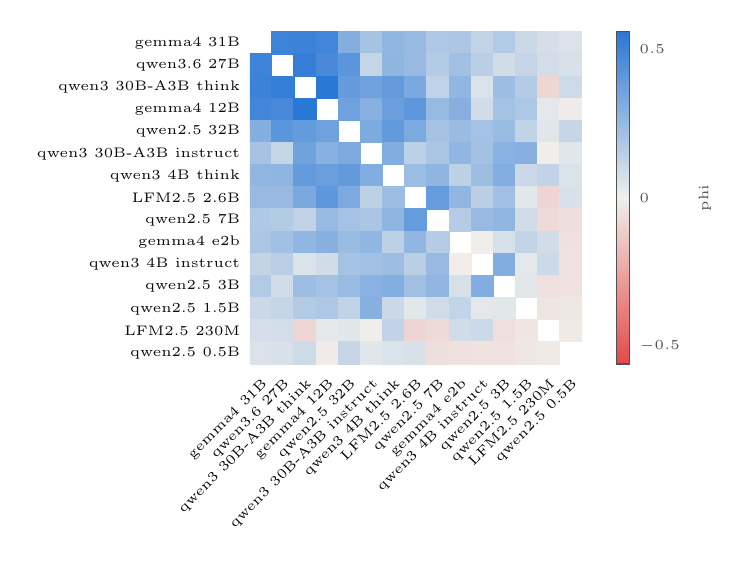
\begin{tikzpicture}
\begin{axis}[
  width=5.8cm, height=5.8cm, enlargelimits=false, colormap name=div,
  point meta min=-0.5592, point meta max=0.5592,
  colorbar, colorbar style={font=\tiny, color=muted, width=5pt,
    ylabel={phi}, ylabel style={font=\tiny}},
  xtick={0,1,2,3,4,5,6,7,8,9,10,11,12,13,14},
  ytick={0,1,2,3,4,5,6,7,8,9,10,11,12,13,14},
  xticklabels={gemma4 31B,qwen3.6 27B,qwen3 30B-A3B think,gemma4 12B,qwen2.5 32B,qwen3 30B-A3B instruct,qwen3 4B think,LFM2.5 2.6B,qwen2.5 7B,gemma4 e2b,qwen3 4B instruct,qwen2.5 3B,qwen2.5 1.5B,LFM2.5 230M,qwen2.5 0.5B},
  yticklabels={gemma4 31B,qwen3.6 27B,qwen3 30B-A3B think,gemma4 12B,qwen2.5 32B,qwen3 30B-A3B instruct,qwen3 4B think,LFM2.5 2.6B,qwen2.5 7B,gemma4 e2b,qwen3 4B instruct,qwen2.5 3B,qwen2.5 1.5B,LFM2.5 230M,qwen2.5 0.5B},
  xticklabel style={rotate=45, anchor=north east, font=\fontsize{4}{5}\selectfont, color=ink},
  yticklabel style={font=\fontsize{4}{5}\selectfont, color=ink},
  tick style={draw=none}, y dir=reverse, axis line style={draw=none},
]
\addplot[matrix plot*, mesh/cols=15, mesh/ordering=rowwise, point meta=explicit] table[meta=v] {
x y v
0 0 nan
1 0 0.5071
2 0 0.5106
3 0 0.4956
4 0 0.3053
5 0 0.2073
6 0 0.2678
7 0 0.2500
8 0 0.1820
9 0 0.1937
10 0 0.1249
11 0 0.1747
12 0 0.1067
13 0 0.0746
14 0 0.0607
0 1 0.5071
1 1 nan
2 1 0.5321
3 1 0.4748
4 1 0.4224
5 1 0.1237
6 1 0.2739
7 1 0.2530
8 1 0.1714
9 1 0.2195
10 1 0.1528
11 1 0.0900
12 1 0.1209
13 1 0.0845
14 1 0.0688
0 2 0.5106
1 2 0.5321
2 2 nan
3 2 0.5592
4 2 0.3972
5 2 0.3607
6 2 0.3973
7 2 0.3338
8 2 0.1361
9 2 0.2683
10 2 0.0614
11 2 0.2340
12 2 0.1719
13 2 -0.0823
14 2 0.0978
0 3 0.4956
1 3 0.4748
2 3 0.5592
3 3 nan
4 3 0.3655
5 3 0.2950
6 3 0.3798
7 3 0.4128
8 3 0.2506
9 3 0.2979
10 3 0.0918
11 3 0.2141
12 3 0.1878
13 3 0.0316
14 3 -0.0149
0 4 0.3053
1 4 0.4224
2 4 0.3972
3 4 0.3655
4 4 nan
5 4 0.3243
6 4 0.3979
7 4 0.3274
8 4 0.2121
9 4 0.2434
10 4 0.2126
11 4 0.2427
12 4 0.1340
13 4 0.0442
14 4 0.1166
0 5 0.2073
1 5 0.1237
2 5 0.3607
3 5 0.2950
4 5 0.3243
5 5 nan
6 5 0.3122
7 5 0.1459
8 5 0.1965
9 5 0.2679
10 5 0.2187
11 5 0.2906
12 5 0.2972
13 5 -0.0015
14 5 0.0413
0 6 0.2678
1 6 0.2739
2 6 0.3973
3 6 0.3798
4 6 0.3979
5 6 0.3122
6 6 nan
7 6 0.2392
8 6 0.2750
9 6 0.1480
10 6 0.2340
11 6 0.3069
12 6 0.1080
13 6 0.1311
14 6 0.0614
0 7 0.2500
1 7 0.2530
2 7 0.3338
3 7 0.4128
4 7 0.3274
5 7 0.1459
6 7 0.2392
7 7 nan
8 7 0.3928
9 7 0.2699
10 7 0.1543
11 7 0.2256
12 7 0.0399
13 7 -0.0862
14 7 0.0691
0 8 0.1820
1 8 0.1714
2 8 0.1361
3 8 0.2506
4 8 0.2121
5 8 0.1965
6 8 0.2750
7 8 0.3928
8 8 nan
9 8 0.1640
10 8 0.2527
11 8 0.2706
12 8 0.0903
13 8 -0.0678
14 8 -0.0552
0 9 0.1937
1 9 0.2195
2 9 0.2683
3 9 0.2979
4 9 0.2434
5 9 0.2679
6 9 0.1480
7 9 0.2699
8 9 0.1640
9 9 nan
10 9 -0.0048
11 9 0.0730
12 9 0.1289
13 9 0.0902
14 9 -0.0466
0 10 0.1249
1 10 0.1528
2 10 0.0614
3 10 0.0918
4 10 0.2126
5 10 0.2187
6 10 0.2340
7 10 0.1543
8 10 0.2527
9 10 -0.0048
10 10 nan
11 10 0.3105
12 10 0.0343
13 10 0.1016
14 10 -0.0436
0 11 0.1747
1 11 0.0900
2 11 0.2340
3 11 0.2141
4 11 0.2427
5 11 0.2906
6 11 0.3069
7 11 0.2256
8 11 0.2706
9 11 0.0730
10 11 0.3105
11 11 nan
12 11 0.0402
13 11 -0.0517
14 11 -0.0420
0 12 0.1067
1 12 0.1209
2 12 0.1719
3 12 0.1878
4 12 0.1340
5 12 0.2972
6 12 0.1080
7 12 0.0399
8 12 0.0903
9 12 0.1289
10 12 0.0343
11 12 0.0402
12 12 nan
13 12 -0.0315
14 12 -0.0257
0 13 0.0746
1 13 0.0845
2 13 -0.0823
3 13 0.0316
4 13 0.0442
5 13 -0.0015
6 13 0.1311
7 13 -0.0862
8 13 -0.0678
9 13 0.0902
10 13 0.1016
11 13 -0.0517
12 13 -0.0315
13 13 nan
14 13 -0.0179
0 14 0.0607
1 14 0.0688
2 14 0.0978
3 14 -0.0149
4 14 0.1166
5 14 0.0413
6 14 0.0614
7 14 0.0691
8 14 -0.0552
9 14 -0.0466
10 14 -0.0436
11 14 -0.0420
12 14 -0.0257
13 14 -0.0179
14 14 nan
};
\end{axis}
\end{tikzpicture}
  \caption{Whether two models miss the same questions, as the phi correlation of their per-question outcomes. Phi is used rather than raw overlap so that two weak models failing nearly everything do not agree trivially. The diagonal is blank.}
  \label{fig:co-failure}
\end{figure}













% Bibliography entries for the entire Anthology, followed by custom entries
%\bibliography{custom,anthology-overleaf-1,anthology-overleaf-2}

% Custom bibliography entries only
\bibliography{custom}

%\appendix

%\section{Example Appendix}
%\label{sec:appendix}

%This is an appendix.

\end{document}
